\documentclass{tufte-handout}
\usepackage{graphicx}
\graphicspath{ {./img/} }

\title{Chapter 2: Operating System Structures}
\author{Andr\'es Ponce}

\begin{document}
\maketitle
\begin{abstract}
	An \textit{operating system} allows us to allocate resources
	to a machine. We can use either a graphical environment or 
	all from the \textit{command line}.
\end{abstract}


\section{Operating System Services}
The OS has some key services that it provides:

\begin{itemize}
	\item \textbf{User Interface}: How does the user interact with the system? There 
			have traditionally been two ways, \textbf{command-line interface}, where the 
			user types the commands it wants the computer to execute. There is also the 
			option for a \textbf{user interface}, where the user clicks icons and opens
			graphical programs to run commands and operate the computer.

	\item \textbf{Program Execution}: One of the main functions of an operating system 
			is to load programs into memory and run those programs. One of the main 
			abstractions that the OS provides is to load/execute programs.

	\item \textbf{I/O operations}: For safety reasons, the user seldom interacts directly
			with I/O devices, but the computer has to communicate with the outside. 
			Writing to a network interface or talking with the filesystem maybe should 
			not be left to the user.....

	\item \textbf{Communication}: Sometimes programs need to communicate with each other,
			maybe about error detection through sockets.

	\item \textbf{Error Detection}: When there is an error allocating the resources,
			memory or I/O error, the OS has to be there to detect and correct the error,
			or to halt the system operation.
	\item \textbf{Resource Allocation}: If there are multiple processes, the CPU has 
			to manage the CPU scheduling routines for each process. There are some
			routines to manage the CPU schedule to manage multiple processes.
	\item \textbf{Logging}: If there is an error in your system, then the OS will
			write what happened to some files. Then we can know what is happening 
			in each process.
\end{itemize}

The way we interact with the operating system is also different. In Linux, the main 
way to interact with the computer is through the \textbf{command line interface}, 
where the user types the commands the computer is to execute. Other systems such as
Windows and MacOs intend for the user to to use a graphical environment with icons 
and graphical folders.

\section{System Calls}
When we want our system to perform some action, we will usually specify the filename
to run, and provide it with any arguments necessary. For example, if we were to type

\begin{center}
		\texttt{cp foo.txt bar.txt}
\end{center}
in our terminal, then our OS would know what commands we wanted to run and on which
files to do it. In this example, the \texttt{cp} will \textit{copy} a file 
called \texttt{foo.txt} and copy to another file on the same directory called 
\texttt{bar.txt}.
Even in this simple command, there are multiple system calls going on,
for example we have to open or create the files, then enter a loop which copies the 
lines, which requires even more system calls.

Usually the way that these calls are implemented is through an 
\textbf{Application Programming Interface}. The shell program might make a request to 
the API which then makes the system call. The reason for this is mostly to provide a 
standard format for systems using the same interface. For example, systems all using
the POSIX standard can all expect similar functionality from its function calls.

When our API runs a command, how do we pass the information that the OS requires?
There are two common approaches: \textbf{register method} and \textbf{block method}.
On Linux, if there are 5 or fewer parameters, we store the individual parameters in 
registers. For more arguments, we use the block method. In this method we store all the
parameters in a block in memory and pass the address of the block. We can also use 
a stack to pass the arguments, since stacks don't care about the size or number
of the arguments.

\subsection{Types of System Calls}
There are six major categories of system calls: \textbf{process control}, 
\textbf{file management}, \textbf{device management},\textbf{information maintenance},
\textbf{communications} and \textbf{protection}.

\begin{enumerate}
	\item \textbf{Process Control}: This are the calls responsible for running 
			programs. If the program terminates normally or abnormally, we will
			generate an appropriate error message. The system might generate a 
			memory dump and place the results in a file for the program to check.

			In programs involving system calls, we have to call direct system calls
			from inside our program. For example, if we have a \texttt{printf()} 
			instruction, we might have to call the equivalent \texttt{write()}
			system call. This type of processes could also apply when we want to 
			\textbf{lock} a certian resource, or prevent its modification until 
			a later point in time.

	\item \textbf{File Management}: When we interact with files, we might also need 
			to create, close, modify, move, etc... files around the directory 
			if we have one.
	\item \textbf{Device Management}: When we have to interact with another device
			such as disk, we have to ask for control of the device first, then
			we can read the data, and finally close the connection. Since these
			functions are similar to the ones used for files, some OSes (Linux) 
			combine the two into one. This means that devices are treated as files.
			The data from one device might be available directly somewhere on the 
			file system!
	\item \textbf{Information Maintenance}: There are also system calls for getting
			information about the system. For example, we can get the \texttt{date()}
			or \texttt{time()}, how much free space there is on the system, etc... 
			These sytem calls are useful for debugging and knowing what order of 
			system calls are being executed. We can use a CPU's \textbf{single step}
			mode to find the order of instructions being executed.
	\item \textbf{Communication}: A common theme is that we need to allow 
			different programs to communicate with each other. We alaready saw some
			general model of how to do this, either with a shared memory model or 
			registers. How do we identify the program we want to talk to?

			Each program gets a unique \textbf{process name} and 
			\textbf{host name}, which will pass a message along. \textbf{Daemons}
			are programs that accept connections from a client.

	\item \textbf{Protection}: When computers had multiple users, it was important
			for the system to control resource allocation among the users. Now, with 
			the Internet the OS still has to control how resources are alocated
			and how we protect the sytem.
\end{enumerate}
\section{System Services}
Some of the functionality that we have come to expect in an operating system includes
file management, networking and communication, program loading and execution.

\textbf{Services} or \textbf{daemons} are programs that usually run in the background.
These programs might wait for requests, such as network managers, and others might 
be monitoring processes.

\section{Linkers and Loaders}
Whenever we run a program, we have to first compile the source file into some object 
file such as \texttt{a.out} or \texttt{a.exe}. The compiler will take the source 
file and make an output file with the name as the previous one.

It is the job of a linker to include any other code necessary in a source file,
for example if we include \texttt{math.h}, the linker is responsible for making 
a coherent file that we can run, with all the references to the pieces of code 
in the correct places. 

When we then type the executable name in the command prompt, we then create a new 
process for the program to run in. We normally assume that the file was all linked
and that all the required libraries were incorporated into the executable file. 
However, on Windowd \textbf{dynamically linked libraries} are only loaded conditionally
if they are needed by the program.

Once we have the final executable file, inside there will a \textbf{symbol table} where
we will have the address for the first instruction and maybe info on the functions
and variables.

\section{Why Are Applications Operating System Specific?}

Application files will usually have some system calls which are unique to the operating
system it's being run on. Some interpreted languages such as Python will read one
instruction at a time, and execute the corresponding instruction on the host machine. 
This would solve the problem for the programmer, who could write a single program
and leave the actual implementation to the interpreter. The interpreter could then 
run on many different environments. 
\footnote{The Executable and Linkable Format \textbf{ELF} is used by most UNIX 
varieties. This format specifies how the function/variable metadata is structured
and stores the address of the starting point for our program.}

Another solution, offered by languages like Java, includes running an entire RTE in 
the form of a virtual machine, where we sometimes transform the code into an 
intermediate language. Then the same source code could run on mulitple systems, 
but likewise the performance will be impacted. 

Once we have an executable file, the operating system expects a certain structure
for the files, with elements that are a certain size, and even the CPU might only 
accept instructions of a different type.\footnote{I'm not sure if this is more of an 
ISA problem or an OS one. But then again, every OS is built to use a certain 
ISA, right?}

APIs specify the available functions at the application layer, meaning that the 
programmer can interact directly with them. However, when dealing at the binary
layer, we need an interface for the program's binary code to deal with 
the OS on a given OS. This is the job of the \textbf{application binary interface}.
The ABI specifies instruction width and other low level details such as how to 
pass the parameters to some functions (remember we have two methods), size of data types
and format of libraries.

\section{OS Design And Implementation}
Although there is on general way to implement an operating system, we can agree on some
general implementation principles.
\footnote{The \textbf{policy} refers to \textit{what} to do, while the \textbf{mechanism}
 refers to \textit{what} to do.}

 Nowadays, OSes are mostly written in C, C++, and assembly for the lower-level parts.
 Other systems such as Android will mix C, assembly and even Java. The disadvantages 
 are of course the speed of the higher-level language.
 \section{OS Structure}
 Operating Systems are usually implemented in individual models, which are clearly 
 defined pieces of code. 

 \begin{marginfigure}
	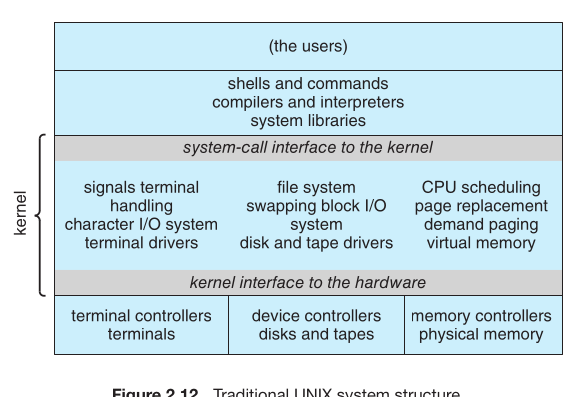
\includegraphics[scale=0.3]{OS_structure.png}
	\caption{The structure of a traditional UNIX system.}
\end{marginfigure}


\subsection{Monolithic Structure}
This type of OS structure involves just placing all the kernel into a single 
binary file. There are no single modules that are loaded individually, but 
instead all the kernel functionality is placed directly in one binary executable.
For the original UNIX, all the filesystem, drivers, CPU scheduling existed in the
kernel itself. For Windows this is still the way to go today. 

Both Windows, Linux, and UNIX have some traces of monolithic kernel design still 
left, however they also combine a layered and modular design. 

The main benefit of a monolithic kernel is the reduced overhead and thus the increase
in speed. This is why popular OSes still contain some trace of monolithic kernel design.
The main drawback is how hard they are to maintain and expand.

\subsection{Layered Approach}
With a layered approach, each layer $m$ might be responsible for a set of data structures
and functions that interact with upper and lower layers. Upper layers have to be 
able to communicate with it, while it has to be able to communicate with lower layers.

While these sorts of layers have successfully been applied to computer networks, 
for operating systems they increase the amount of overhead. This is due to the 
traversal of many layers to obtain some service. Also clearly defining the 
function of a single layer can be complex.

\subsection{Microkernel}
Yet another approach to OS design is the microkernel, in which many non-essential 
kernel functions are removed and instead treated as user programs. For example, the
drivers and file system might be placed outside the kernel. The result is a kernel 
that is a lot smaller and uses a lot less memory. The \textbf{Darwin} microkernel,
used in MacOS might be the most famous example of microkernel.

Again, the biggest drawback is the overhead involved in having two parts of the 
OS communicate when the message have to go through the microkernel before there is some
context switching happening.

\subsection{Modules}
The most effective way we can handle the kernel might be to have a kernel that 
handles the most basic functions, such as scheduling and the file system. Then,
during boot time or run time we can dynamically load modules we need. This approach
reduces the hassle since we avoid compiling the kernel every time we want to load
a new module.

\section{Building and Booting an Operating System}
How do we get an OS running? We might already have one installed on our computer
at the time of purchase, but we will focus on the case where we don't have one.
We would have to write the source code and then compile it for our current system.
We could do it by modifying the \texttt{config} file and tailor the settings to our
build.

For the Linux kernel, we can follow something resembling these steps:
\begin{enumerate}
	\item Download the source code from \texttt{http://www.kernel.org}
	\item Run \texttt{make menuconfig} to generate the \texttt{.config} file
			that holds our settings.
	\item Run \texttt{make} to compile the main kernel with the \texttt{.config} file
			we have aleready generated.
	\item Run \texttt{make modules} to compile the modules.
	\item Run \texttt{make modules\_install} to install the modules on the kernel.
	\item Finally, install the kernel by running \texttt{make install} and reboot.
\end{enumerate}

\section{System Boot}
What happens when we press the power switch and turn the computer on? First, we 
run a program called a \textbf{boot loader} which is in charge of locating the 
kernel to be loaded, loading it into memory. The kernel then initializes the hardware
and mounts the root file system.

When the system is first turned on \footnote{ayyyy}, an initial bootloader is loaded
from non-volatile memory.This initial boot loader might then load another boot loader
such as GRUB from the \texttt{/boot} section of the disk. This next boot loader might
then locate the kernel or allow the user to choose from many kernels. This boot 
loader must be small enough to fit in the determined boot section of the disk.

The Linux image is a compressed file which is decompressed when it is loaded into
memory. This is done to speed up the boot process.
\footnote{The boot loader will also create a separate RAM environment known as 
\texttt{initramfs}, which loads the necessary drivers and kernel modules to load the
OG kernel.}
Then we mount the actual file system on the correct place.

\section{Operating System Debugging}
How can we fix problems occuring during the kernel execution? When there is a problem
in the kernel, we will usually write the contents of the memory to a section of the 
disk that does not contain a file system. This way, we can probe the code with a 
debugger.

A big part of debugging involves finding \textbf{performance bottlenecks}. To do this,
the OS has to provide some way of measuring performance either by process or 
system-wide. There are two methods: \textbf{counters} and \textbf{tracers}.

\textbf{Counters} will keep track of how much resources either a single process 
is using or how much resources are being used at a system level. In Linux, the details
for process usage is stored in \texttt{/proc}, where each subdirectory indicates a 
single process id and its statistics.

\textbf{Tracing} involves looking at the steps involved in system call invocations.
\end{document}
